\chapter{Conclusão}

Os métodos geoestatísticos de estimativa e simulação de teores requerem a delimitação prévia de domínios estacionários para modelagem do depósito mineral. Na indústria da mineração, modelos geológicos determinísticos são amplamente utilizados. No entanto, esses modelos não permitem a avaliação da incerteza em volumes e toneladas. A geometria dos domínios geológicos afeta diretamente a avaliação dos recursos minerais, pois determina os volumes de minério e estéril disponíveis e pode ser responsável pelas maiores incertezas em um projeto de mineração. Assim, o impacto é significativo na estimativa da tonelagem de minério, levando a estimativas enviesadas, erros no planejamento de lavra, custos inesperados na operação e desvios nas receitas esperadas \cite{srivastava2005probabilistic}.

Além da variável categórica, o banco de dados \textit{Swiss Jura} apresenta 6 variáveis contínuas que representam o teor de diferentes metais (Cr, Ni, Zn, Cd, Cu e Pb) em ppm. A \autoref{jura_cr} mostra o mapa de amostras para a variável Cr em \autoref{pts} e mostra em \autoref{cr_argo} os teores de Cr em ppm estimados por krigagem ordinária no domínio Argovian definido na \autoref{quartenary_model}. A linha vermelha da \autoref{risk_anal} mostra o conteúdo metálico de Cr considerando a espessura em Z dos blocos como 1 metro e a densidade 5g/cm³ para simplificar os cálculos.

\begin{figure}[H]
    \caption{Variável Cr do \textit{Swiss Jura}} \label{jura_cr}
     \centering
     \subfloat[][Mapa de amostras da variável Cr.]{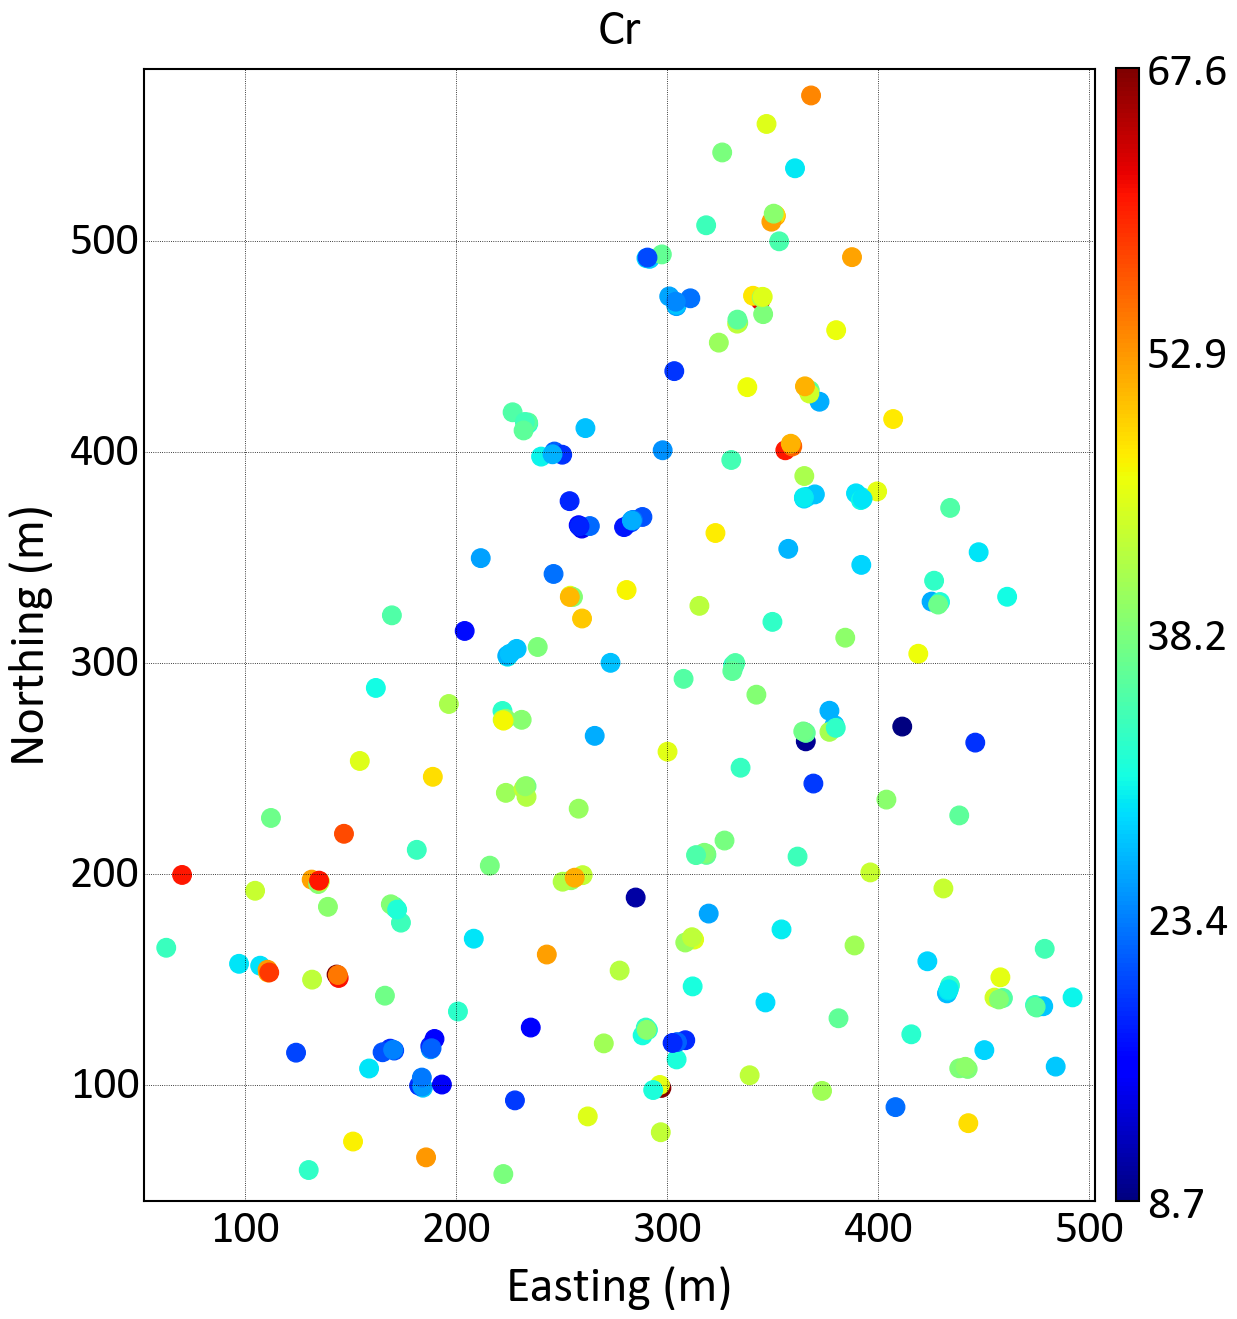
\includegraphics[width=0.45\textwidth]{capitulo_4/imagens/Cr.png}\label{pts}}
     \hspace{1em}
     \subfloat[][Variável Cr estimada por krigagem no domínio Argovian.]{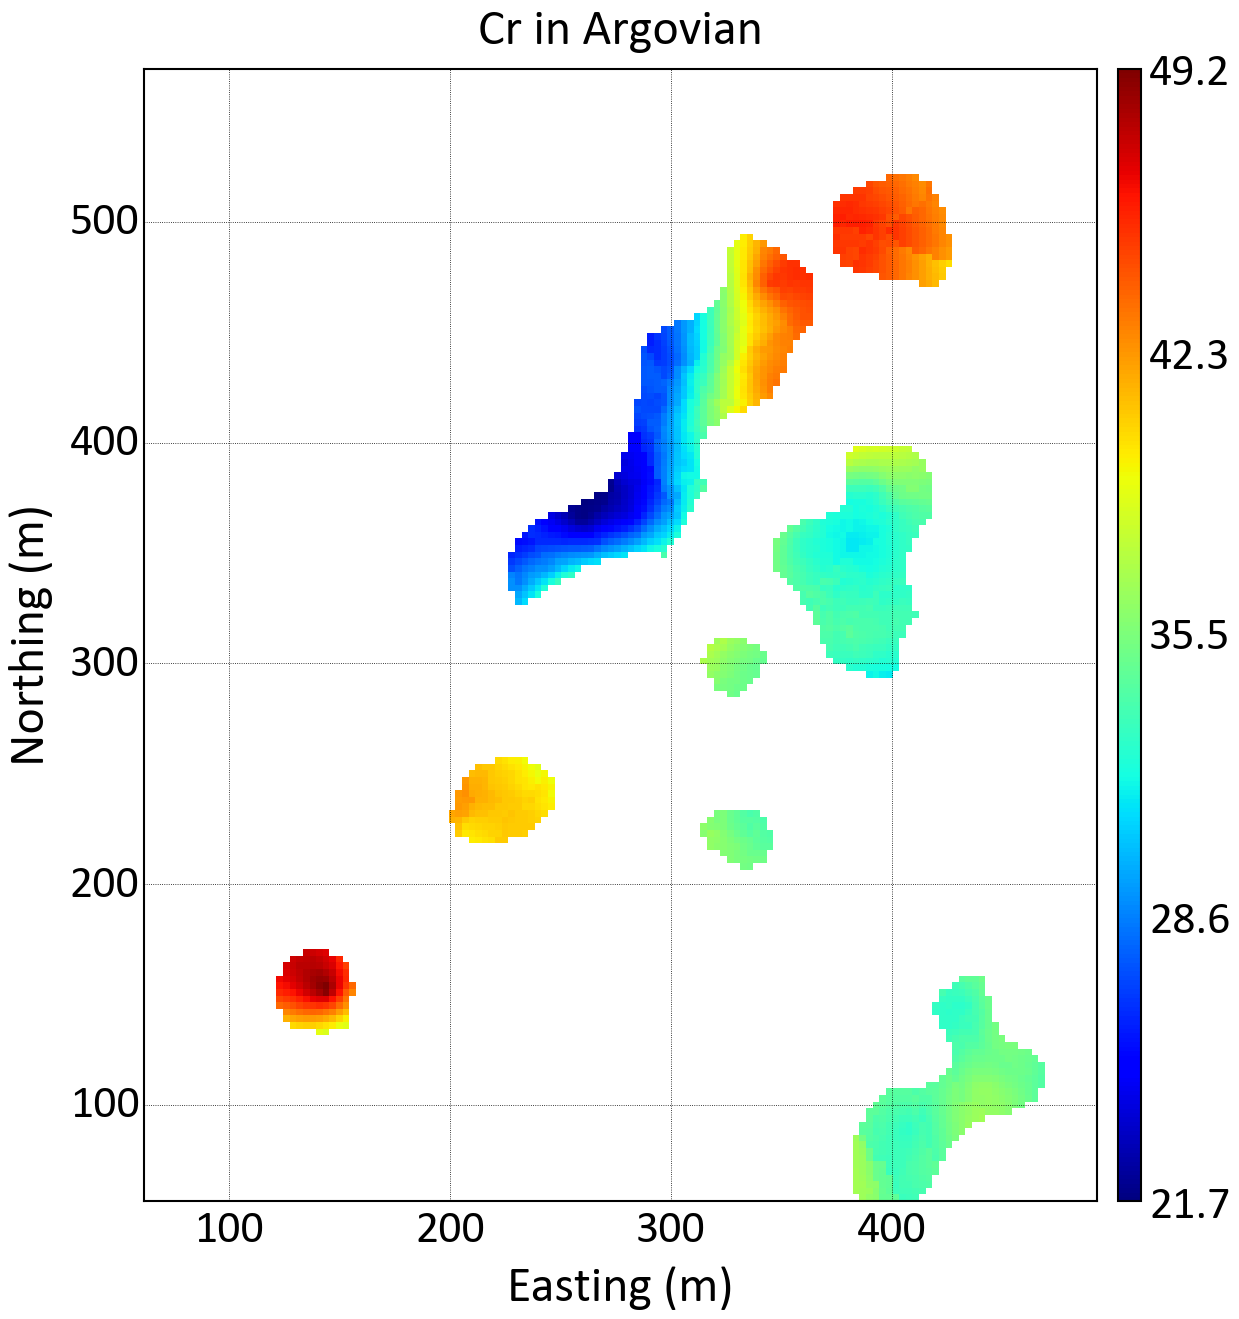
\includegraphics[width=0.45\textwidth]{capitulo_4/imagens/Cr_krig_argovian.png}\label{cr_argo}}
\end{figure}

Foram realizadas 100 realizações para o modelo geológico do \textit{Swiss Jura} usando a metodologia apresentada na \autoref{pfiels_sec}. O conteúdo metálico de Cr foi calculado para cada uma das realizações para o domínio Argovian e o resultado é mostrado no histograma da \autoref{risk_anal}.

\begin{figure}[H]
\caption{Análise de risco para o conteúdo metálico de Cr no domínio Argovian.}
\label{risk_anal}
\centering
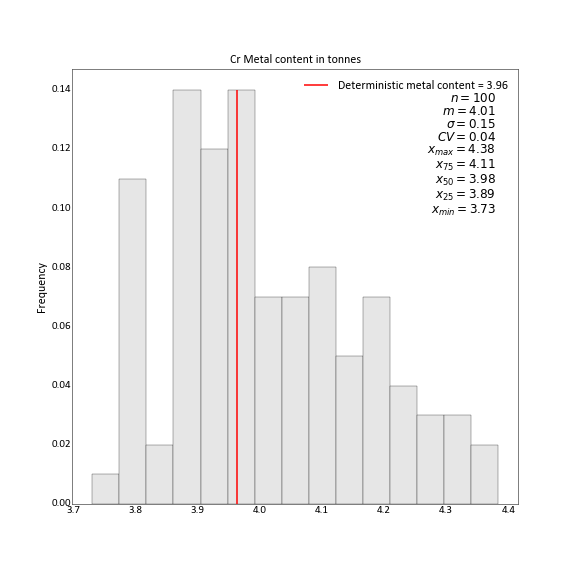
\includegraphics[width=0.8\textwidth]{capitulo_4/imagens/metal_content.png}
\end{figure}

A partir da análise de risco em relação ao conteúdo metálico de Cr, levando em consideração somente a incerteza em relação ao modelo geológico, no domínio Argovian há possibilidade de que haja disponível um mínimo de 3.7 toneladas de Cr e um máximo de 4.3 toneladas de Cr. Uma variação percentual de 17,5\% em massa que deve ser levada em consideração na fase de planejamento mineiro.

Dos três métodos propostos e investigados nessa tese para avaliação de incerteza em modelos geológicos usando funções distância assinaladas, dois são baseados em simulações gaussianas não condicionais e um deles não envolve simulação, apenas interpolações.

Por ser baseado em interpolação global, o método baseado na parametrização do suporte do \textit{kernel} gera modelos que apresentam contatos suaves que são geologicamente realistas. Os outros dois métodos baseados em simulação, apesar de apresentarem semelhanças, têm características distintas. A avaliação de incerteza usando campos de probabilidade e funções distância assinaladas é consideravelmente mais simples do que a simulação hierárquica de contatos. Entretanto, apresenta algumas limitações e desvantagens. Ao contrário da simulação hierárquica de contatos, a zona de incerteza deve ter a mesma espessura ao redor de todos os contatos. Além disso, também ao contrário da simulação hierárquica dos contatos, um único variograma para a simulação não condicional deve representar os contatos entre todas as diferentes categorias do depósito mineral. Embora no estudo de caso apresentado nessa tese os contatos gerados pelos campos potenciais tenham sido suaves e realistas algumas combinações de parâmetros podem gerar contatos desconexos e irreais. O mesmo não acontece com a simulação hierárquica de contatos, a comparação do valor simulado com o interpolado bloco a bloco faz com que os contatos sejam contínuos tornando o método robusto no sentido de criar contatos realistas.

Embora os métodos propostos criem modelos realistas de forma rápida e direta eles não devem ser aplicados a todos os tipos de depósito de forma indiscriminada. Nenhum dos métodos leva em consideração elementos estruturais da geologia e também não dão tratamento diferenciados para estruturas específicas como dobras, diques, falhas ou lentes. A reprodução desse tipo de estrutura por métodos de modelagem geológica automáticos geralmente não é satisfatória. Entretanto, os métodos propostos podem ser aplicados em fases iniciais da pesquisa mineral, para bancos de dados em 2D, para depósitos de baixa complexidade geológica, para depósitos de média complexidade geológica e alta densidade amostral ou podem ainda ter suas realizações refinadas manualmente por um geomodelador experiente poupando tempo e esforço do profissional.  

A validação de realizações para o modelo geológico é especialmente difícil. Nessa tese apenas a reprodução das amostras e checagem visual de seções foram aplicadas. Caso haja confiança de que a amostragem seja representativa das proporções de cada uma das litologias no depósito mineral ainda é possível verificar sua reprodução. A reprodução dos variogramas dos indicadores para todas as categorias de um modelo multi-categórico de forma simultânea é um evento raro mesmo em bancos de dados de geometria simples em 2D. As estruturas geológicas, muitas vezes, são curvilineares e sua continuidade espacial não pode ser capturada por variogramas "tradicionais". A modelagem implícita tende a gerar estruturas em formatos circulares ("\textit{blobs}") ao redor das amostras, e em forma de salsicha em torno de furos de sondagem. O surgimento desse tipo de estrutura indica que os modelos não são satisfatórios e alguma mudança nos parâmetros deve ser feita.

\section{Sugestões para trabalhos futuros}

Dada a limitação de tempo para conclusão da tese algumas ideias e aprimoramentos foram deixados para trabalhos futuros. 

 \begin{itemize}
    \item Definir uma metodologia para determinar os variogramas das simulações não condicionais nos métodos dos campos potenciais e simulação hierárquica; 
    \item Definir uma metodologia objetiva para calibrar a zona de incerteza nos métodos dos campos potenciais e simulação hierárquica. A zona de incerteza não necessariamente deve ser simétrica ao redor dos contatos. Não devem haver amostras no interior da zona de incerteza;
    \item Aprimorar a parametrização do suporte do \textit{kernel} para que a sensibilidade ao parâmetro fmin seja reduzida;
    \item Conduzir uma análise de risco mais robusta com simulação de teores e do modelo geológico em um banco de dados real comparando os resultados com os teores krigados em um modelo geológico determinístico; 
    \item Desenvolver uma metodologia para validação dos modelos geológicos. Usar redes neurais treinadas em seções de modelos determinísticos para identificar estruturas contínuas e realistas é uma avenida de investigação;
    \item Desenvolver metodologias, ou adaptações de metodologias existentes, para modelar estruturas geológicas especĩficas (dobras, diques, falhas, lentes) e avaliar sua incerteza.
 \end{itemize}